\capitulo{5}{Aspectos relevantes del desarrollo del proyecto}

En este apartado vamos a recoger los aspectos importantes que han ocurrido a lo largo del desarrollo del proyecto. Incluyendo las decisiones tomadas, los cambios en el proyecto o los problemas que hayan podido surgir y las soluciones que se han planteado (si se consiguió solucionar.)

\section{Inicios del proyecto}
La idea de trabajar en este proyecto de la búsqueda de ampliación de los conocimientos adquiridos a lo largo de la carrera. Ya poseía algún conocimiento superficial sobre el Web Scraping y sus métodos, es por eso por lo que parecía una idea interesante profundizar en esta materia. Además, la idea propuesta por el tutor se postulaba como adecuada a mis necesidades y asequible en los marcos de tiempo que se disponía.

Tras formalizarse los objetivos del proyecto y las metodologías de trabajo se pone en marcha el proyecto el \emph{5/11/18}.

\begin{figure}[H]
	\centering
	
\includegraphics[width=0.4\textwidth]{logo_150}
	\caption{Logo de PCVN.}
	\label{fig:logo}
\end{figure}


\section{Metodologías}
En la formalización del proyecto se utilizaría una metodología ágil basada en Sprints(Metodología Scrum), de desarrollo incremental con revisiones.
\begin{itemize}
	\item	Se estableció que la duración de los Sprints sería de una semana
	\item	Los objetivos para el inicio se marcarían semanalmente, revisando lo conseguido en el sprint anterior
	\item	Se realizarían reuniones semanales, (siempre y cuando las circunstancias lo permitieran).
\end{itemize}

En líneas generales creo que los resultados de esta metodología han sido satisfactorios y que han tenido un impacto muy positivo en el proyecto.

\section{Toma de decisiones}
\subsection{Páginas Web}
En la formalización del proyecto también se declaró cual serían las páginas de las cuales se procedería a extraer la información. Por su relevancia y número de datos almacenados se decidió que se usaría:
\begin{itemize}
	\item Google Scholar.
	\item Scopus.
	\item Web of Science.
	
\end{itemize}

\section{Formato de almacenamiento}
Una de las decisiones más importantes a tomar en el proyecto, es como se guardaría toda la información recolectada para ser posteriormente tratada. Se plantearon tres alternativas
\subsection{BibTeX .}
	\begin{figure}[H]
		\centering
		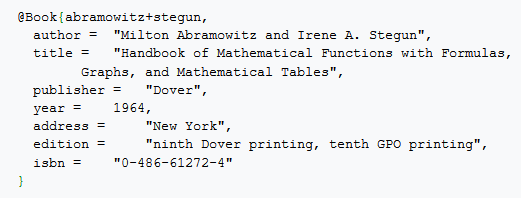
\includegraphics[width=1\textwidth]{bibtex2}
		\caption{Imagen de ejemplo de una publicación en formato BibTeX.}
		\label{fig:bibtex2}
	\end{figure}
	
\subsection{EndNote.}
	\begin{figure}[H]
		\centering
		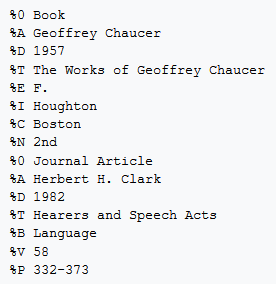
\includegraphics[width=0.7\textwidth]{endnote}
		\caption{Imagen de ejemplo de una publicación en formato EndNote.}
		\label{fig:endnote}
	\end{figure}

\subsection{RIS.} 
	\begin{figure}[H]
		\centering
		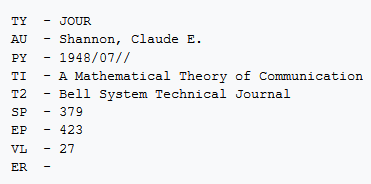
\includegraphics[width=0.7\textwidth]{ris}
		\caption{Imagen de ejemplo de una publicación en formato RIS.}
		\label{fig:ris}
	\end{figure}
	
Todos son formatos de bibliografía basados en etiquetas y valor, en las que a la etiqueta representa un campo (Ej. Autor, Título) y el valor de dicho campo (Ej. Roberto Poza, PCVN)

 	Aunque todos los formatos podrían ser perfectamente a la estructura de diccionarios de \emph {Python}, finalmente se optó por usar el formato BibTeX pues las etiquetas correspondientes al campo son más explicativas y se adaptaban mejor a la propia estructura devuelta por las librerías, además las librerías para trabajar con este formato eran más numerosas y con amplia experiencia y documentación.

\section{Librerías para la extracción de datos}
Tras una toma de contacto con las técnicas de \emph{Web Scraping} y las páginas de donde se sacaría esta información se procedió a determinar de qué forma se podría trabajar con esta información.
\begin{itemize}
	\item Scholarly: Para la obtención de los datos de \emph{Google Scholar}.
	\item Python-Scopus: Para la obtención de los datos de \emph{Scopus} .
	\item Selenium: Para la obtenciones los datos De \emph{Web of Science}.
\end{itemize}

\section{Interfaz de usuario del proyecto}
Se tenía la idea de dotar al proyecto de una interfaz, para que el contacto con el usuario no tuviera que ser a través de  la línea de comandos. Se barajo la posibilidad de utilizar una interfaz basada en texto \emph{TUI} o bien una interfaz gráfica \emph{GUI}, finalmente se optó por esta última pues el esfuerzo extra que requería para su realización era aceptable y se entiendo que merecía la pena para ofrecer una mejor experiencia al usuario.
 	Finalmente se usó la librería Tkinter para desarrollar esta interfaz, que si bien es sencilla es bastante funcional.
\begin{figure}[H]
	\centering
	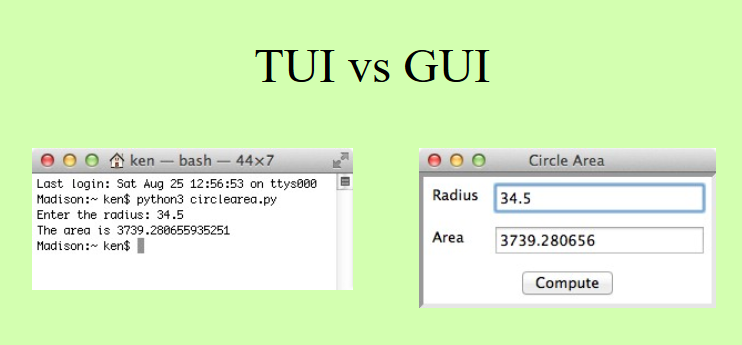
\includegraphics[width=1\textwidth]{tuivsgui}
	\caption{Imagen de ejemplo de una interfaz TUI vs GUI.}
	\label{fig:tuivsgui}
\end{figure}
\section{Problemas encontrados}
\subsection{Función Google Scholar}
En un principio se pretendió implementar una función que permitiera calcular cuantas de las citas de un artículo no eran auto citas, para esto se debía localizar cual eran las publicaciones que citaban la actual publicación y reconocer si alguno de los autores de la publicación citada se encontraba en la publicación citadora. Sin embargo la función encargada de devolver los datos de las publicaciones citadores parecía sufrir algún tipo de problema pues no siempre funcionaba correctamente, como resultado se acabó descartando la idea dejando el número de citas tal y como lo devolvía \emph{Google Scholar}
\subsection{Diferencias entre formatos y duplicados}
El archivo \emph{BibTeX} con los datos referentes a \emph{Web of Science} es generado directamente por la propia página web con lo que carecía del mismo formato que el generado por la librería \emph{Bibtexparser}, es por eso que se tuvo que crear una función para el tratado de los datos, teniendo que renombrar algunos campos , asi como aplicar filtros de caracteres a otros. Además se aprovechó para a su vez aplicar la detección de publicaciones duplicados por doble factor: Titulo e ISSN.
\subsection{Índice de calidad}
Las publicaciones científicas se pueden dividir de acuerdo a si están indexadas de acuerdo con un índice de calidad relativo o no. En el caso de esta ultimas no existe problema , con los datos extraídos valdría sin embargo para las primeras es necesario más información (\emph{Índice de impacto, posición de la revista en la categoría, tercíl, cuartil}). Es por eso que se tuvo que utilizar la herramienta Selenium para buscar esta información en \emph{JCR InCites} para cada una de las revistas de la lista de publicaciones, se implementó un sistema de listas y diccionarios en el que una vez consultada los datos de una revista se almacenaba la información de todos los años , por si hiciera falta para otra publicación consiguiendo así reducir ligeramente los tiempos de ejecución pero aun así eran bastante elevados.
\begin{figure}[H]
	\centering
	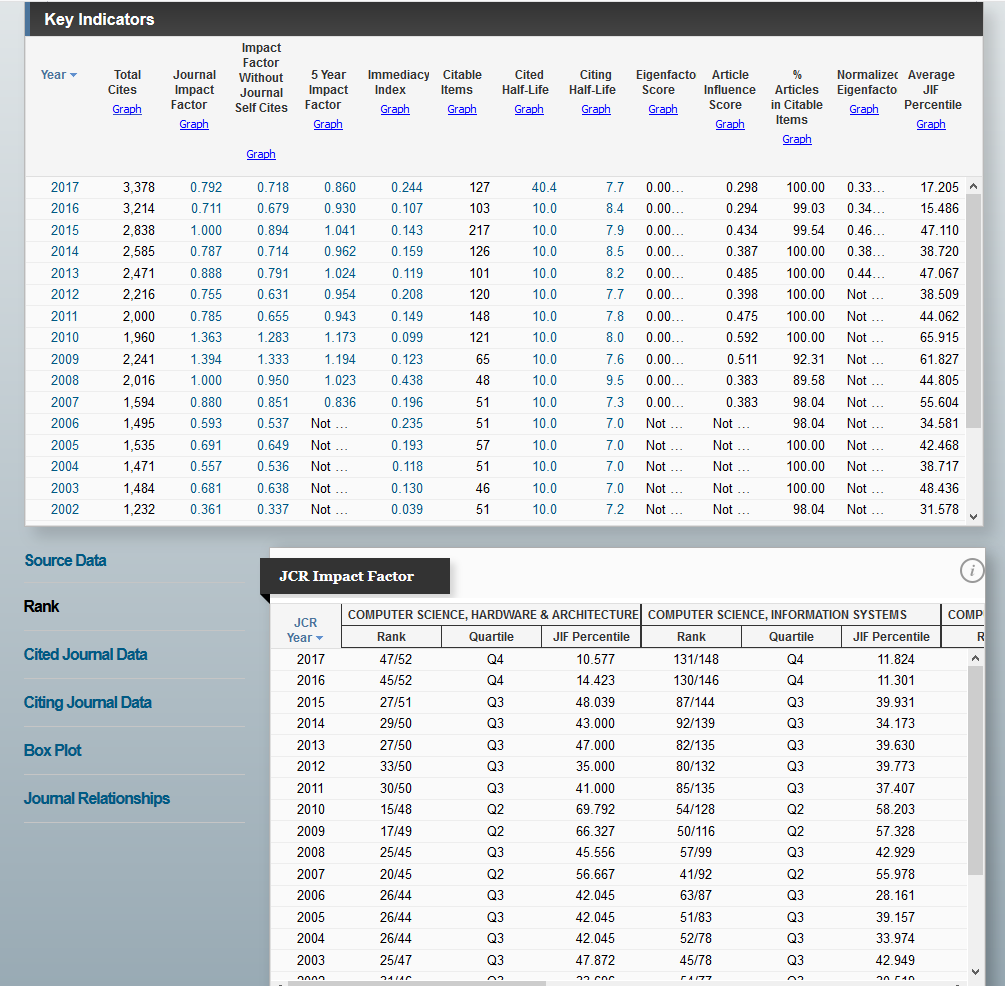
\includegraphics[width=0.8\textwidth]{rank}
	\caption{Imagen de ejemplo de las tablas contenedoras de los indicios de calidad de una publicación.}
	\label{fig:rank}
\end{figure}
\subsection{Tiempo de ejecución en la consulta de índices de impacto}
Como se ha comentado en el apartado anterior, los tiempos de ejecución era aún muy elevado a pesar del sistema de listas y diccionarios implementados. El problema radicaba en que esa información recogida una vez finalizada era perdida, la solución fue bastante simple guardar el objeto Python para que en la siguiente ejecución pudiera ser cargada y utilizada usando la librería \emph{pickle}.
Con esta sencilla solución se consiguió reducir notablemente los tiempos de ejecución.
\subsection{Error en Python-Scopus}
Por algún motivo los resultados arrojados por la librería no estaban completos, en la mayoría de los casos no devolvía los autores de cada publicación, se investigó las peticiones que realizaba y recibía la propia librería, pero no parecía haber nada erróneo por lo que se dedujo que debía ser algún problema con la gestión de las peticiones del propio servidor. Haciendo necesaria una nueva forma de obtener la información.
	Tras una nueva investigación sobre Scopus, se descubrió una opción muy parecida a la que presenta \emph{Web of Science} para exportar la información encontrada a un fichero \emph{BibTeX}, así que se decidió usar de nuevo la herramienta \emph{Selenium} para buscar y exportar la información referente al autor.
\begin{figure}[H]
	\centering
	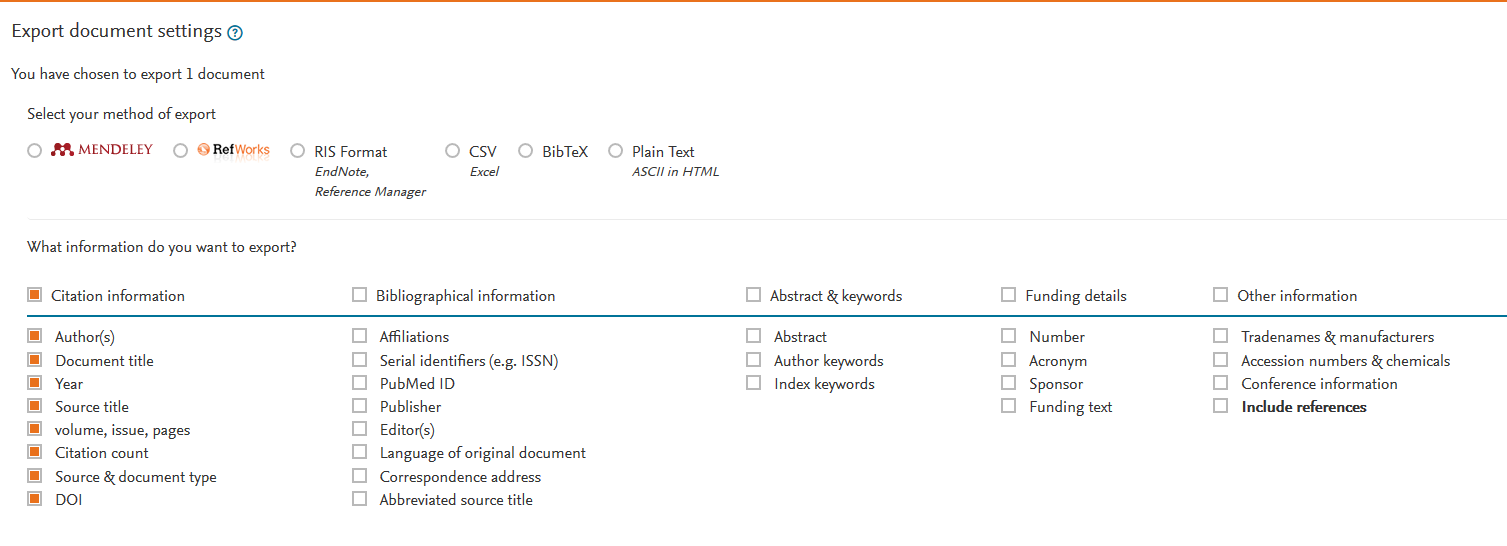
\includegraphics[width=1\textwidth]{export}
	\caption{Imagen que muestra la opción para exportar los datos encontrados al formato elegido en Scopus.}
	\label{fig:export}
\end{figure}
\subsection{Errores con Selenium}
Al realizar el proceso de subida de los datos extraídos y tratados a \emph{ACADEMIA} se producían números fallos de carga de página y otra excepciones , lo que hacía que fallase la ejecución sin posibilidad de recuperarse y finalizando la ejecución de la aplicación. Además, el tiempo que tomaba era demasiado alto. Es por eso que se decidió investigar sobre como el navegador se relacionaba con el servidor para tratar de imitarlo directamente en la aplicación pasando a manejar directamente a mano las peticiones \emph{POST} y \emph{GET} sin necesidad de usar Selenium.

	Para ello se utilizo la herramienta \emph{Burp} , de la cual ya hemos hablado antes y que permite actuar de proxy entre el navegador y el propio servidor, viendo así que peticiones se realizan , con que parámetros y a que direcciones. Se comenzó así un proceso de Ingeniería Inversa para replicar las interacciones generadas por la navegación normal \begin{figure}[H]
	\centering
	
\includegraphics[width=1\textwidth]{burp}
	\caption{Ejemplo de capturas análisis realizado con \emph{Burp}.}
	\label{fig:burp}
\end{figure}
	El primer paso fue estudiar cuales eran los parámetros para el inicio de sesión en la aplicación para realizar la petición \emph{POST} junto con el usuario y la contraseña correspondiente, tras esto se da un proceso de re dirección hasta llegar a la pantalla principal de la aplicación.
\begin{figure}[H]
	\centering
	
\includegraphics[width=1\textwidth]{burp}
	\caption{Análisis de la peticion \emph{POST} para iniciar sesión.}
	\label{fig:burp}
\end{figure}
	El segundo paso consiste en acceder al área del currículo para añadir nuevas publicaciones, en la que solo hace falta una simple petición \emph{GET} a la url correcta para lograrlo.
\begin{figure}[H]
	\centering
	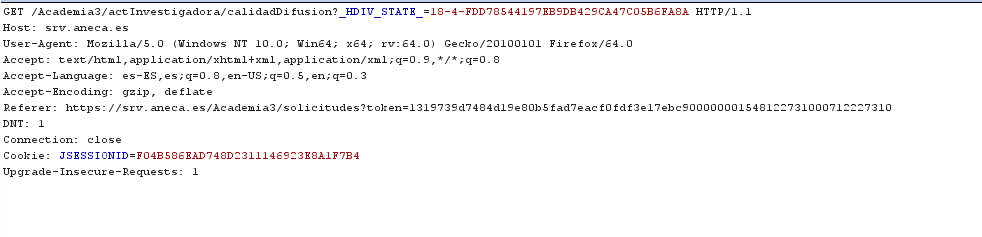
\includegraphics[width=1\textwidth]{burp2paso}
	\caption{Análisis de la peticion \emph{GET} para acceder al \emph{CV}.}
	\label{fig:burp2paso}
\end{figure}
	El tercer paso y el más difícil pues en el parámetro "data" de la petición \emph{POST} para enviar los datos, se incluye una pequeña cadena de texto o \emph{token} creada aleatoriamente para entorpecer las labores de automatización. Sin embargo esta cadena solamente se regenera cuando se realiza una petición \emph{GET} para subir un tipo de publicación , esto quiere decir que para todos los artículos indexados podemos usar el mismo \emph{token} extraído de la respuesta a la petición \emph{GET} del servidor y así con todos los tipos de publicaciones.
\begin{figure}[H]
	\centering
	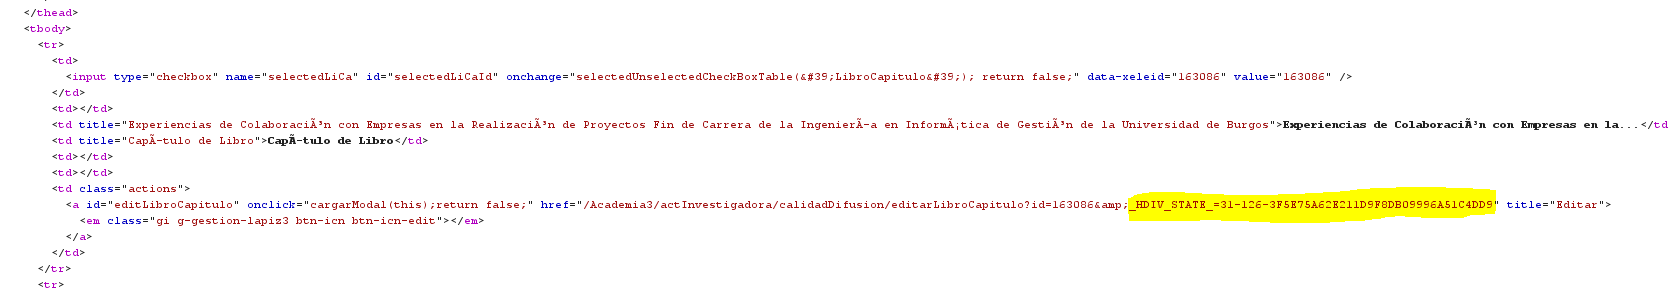
\includegraphics[width=1\textwidth]{burp3paso}
	\caption{Análisis de la respuesta\emph{HTML} a la petición \emph{GET} para añadir publicaciones, en subrayado se encuentra el \emph{token}.}
	\label{fig:burp3paso}
\end{figure}
	Así pues la solución pasa por agrupar todas las publicaciones según su tipo realizar la petición \emph{GET} para poder obtener el \emph{token} y realizar tantas peticiones \emph{POST} , como publicaciones haya en la lista, y repetir este proceso con cada tipo destino de publicación. Burlando así el sistema de entorpecimiento de la automatización.
